%!TEX root=document.tex


\subsection{Pruning-Based Optimizations}
\label{sec:pruning_opt}
In practice, most visualizations are low-utility, meaning computing them wastes computational resources.
Thus, as described earlier, at the end of every phase, 
the execution engine uses pruning optimizations to determine which 
aggregate views to discard.
Specifically, partial results for each view based on the data processed
so far are used to estimate utility and views with low utility are discarded.
The \SeeDB execution engine supports two pruning schemes. The first uses 
confidence-interval techniques to bound utilities of views, while the second uses
multi-armed bandit allocation strategies to find top utility views.





\stitle{Confidence Interval-Based Pruning.}
\label{sec:confidence_interval}
Our first pruning scheme uses worst-case statistical confidence intervals to
bound view utilities.
This technique is similar to top-k based pruning algorithms developed 
in other contexts~\cite{DBLP:conf/vldb/IlyasAE04, DBLP:conf/ICDE/ReDS07}.
Our scheme works as follows: during each phase,
we keep an estimate of the mean utility for every aggregate view $V_i$ and a
confidence interval around that mean.
% That is, for every view $V_i$ we track its mean utility $u_i$, and a
% confidence interval around the mean, $u_i \pm c_i$. 
At the end of a phase, we use the following rule to prune low-utility
views:
{\em If the upper bound of the utility of view $V_i$ is less
than the lower bound of the utility of $k$ or more views, then $V_i$ is discarded.}
To illustrate, suppose a dataset has 4 views $V_1$ \ldots $V_4$ and we want to 
identify the top-$2$ views.
Further suppose that at the end of phase $i$,
$V_1$-$V_4$ have confidence intervals as shown in Figure \ref{fig:conf_interval}.
Views $V_1$ and $V_2$ have the highest utility estimates so far and are
likely to be in the top-$2$ views.
View $V_3$ is currently not the top-$2$, but its confidence interval overlaps
with that of the top-$2$, making it possible that $V_3$ could replace $V_1$ or $V_2$.
The confidence interval for $V_4$, on the other hand, lies entirely below the confidence
intervals of $V_1$ and $V_2$.
Since we can claim with high probability
that the utility of $V_4$ lies within its confidence interval, it follows that,
with high probability, $V_4$'s utility will be lower than that of both $V_1$ and
$V_2$, and it will not appear in the top-$2$ views.
\papertext{Pseudocode for our pruning scheme can be found in our technical report~\cite{seedb-tr}.}
\techreport{We state the algorithm formally in
Algorithm~\ref{algo:ci_based_pruning}.}

\begin{figure}[h]
\vspace{-10pt}
\centerline{
\hbox{\resizebox{4cm}{!}{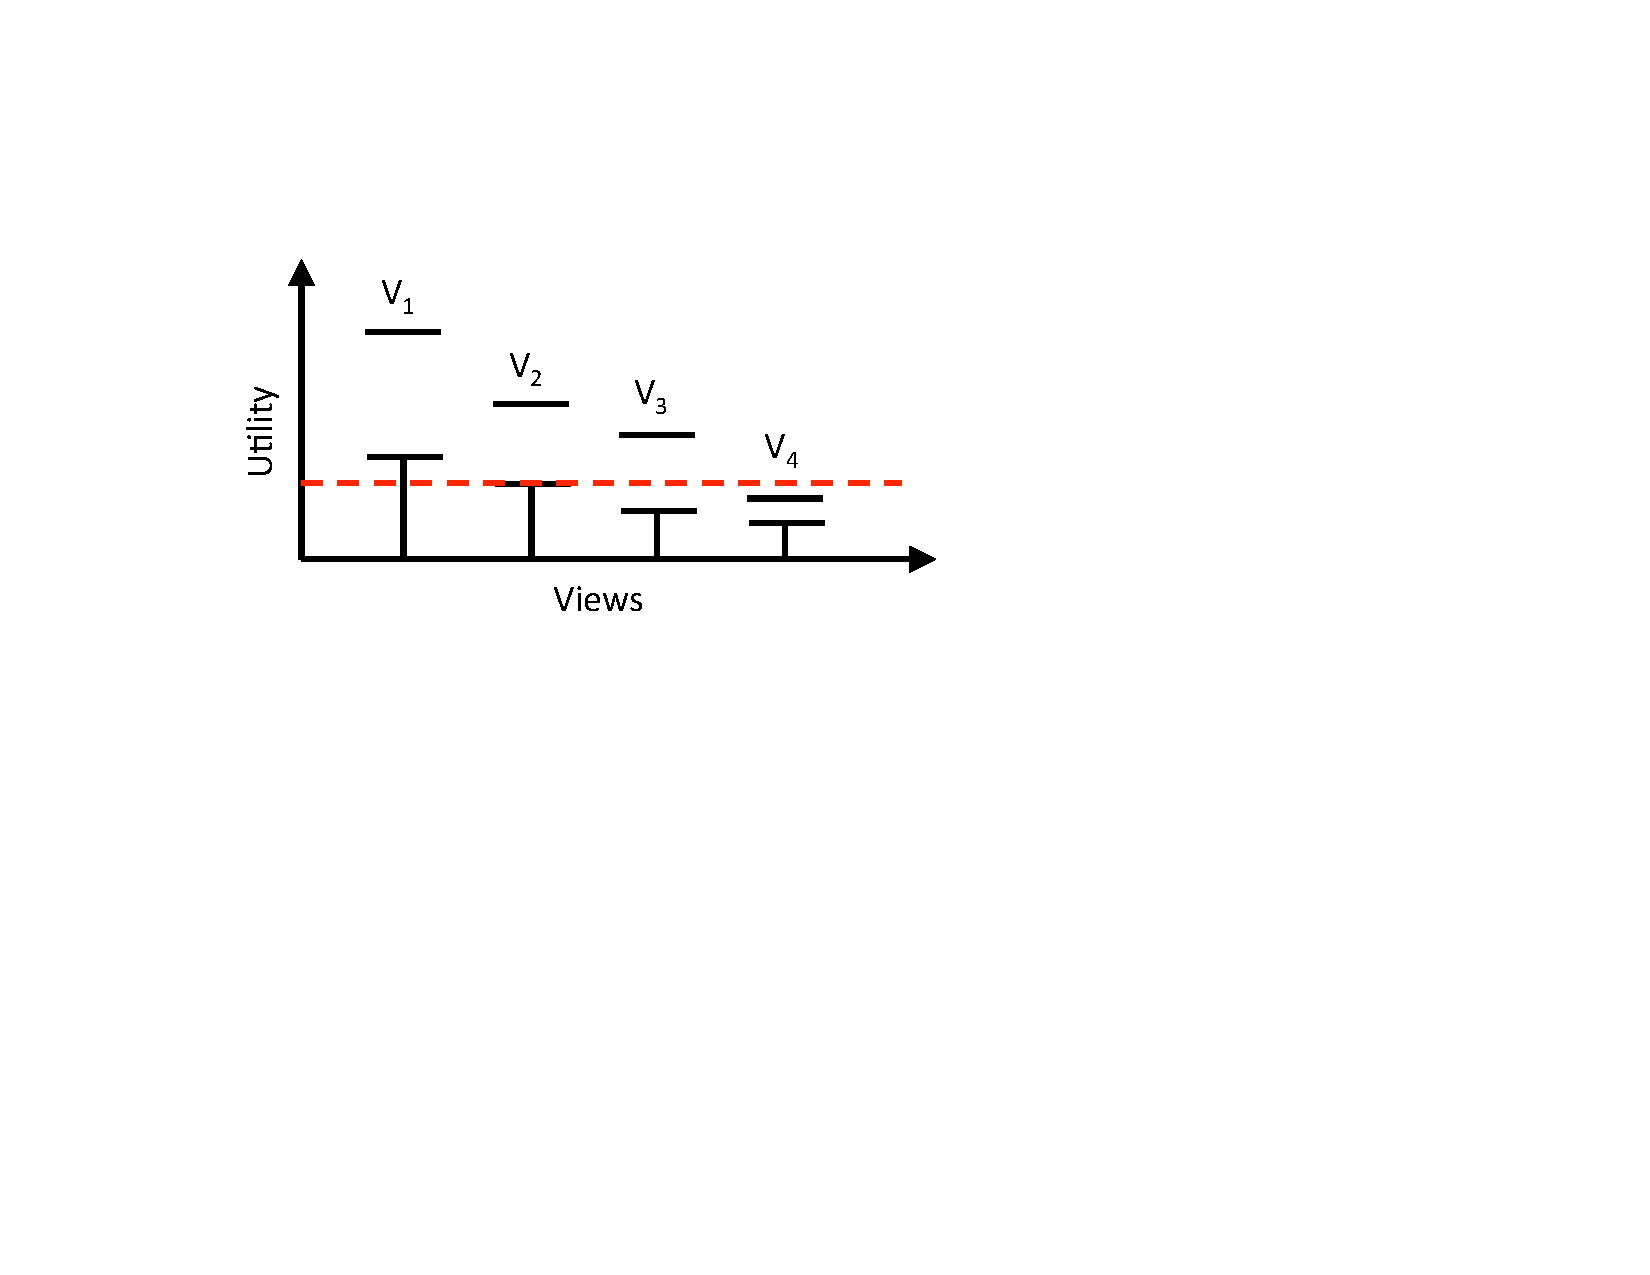
\includegraphics[trim=0mm 0mm 0mm 0mm, 
clip=true]{Images/confidence_pruning.pdf}}}}
\vspace{-10pt}
\caption{Confidence Interval based Pruning}
\label{fig:conf_interval}
\vspace{-10pt}
\end{figure}


\techreport{
\begin{algorithm}
\caption{Confidence Interval Based Pruning}
\label{algo:ci_based_pruning}
\begin{algorithmic}[1]
\State viewsInRunning.sortByUpperbound()
\State topViews $\gets$ viewsInRunning.getTopK()
\State lowestLowerbound $\gets$ min(lowerbound(topViews))
\For {view $\not \in$ topViews}
\If {view.upperbound < lowestLowerbound}
\State viewsInRunning.remove(view)
\EndIf
\EndFor
\end{algorithmic}
\end{algorithm}
}

We use {\it worst case} confidence intervals as derived from
the Hoeffding-Serfling inequality~\cite{serfling1974probability}.
The inequality states that if we are given $N$ values $y_1, \ldots, y_N$ in 
$[0, 1]$ with average $\mu$, and we have have drawn $m$ values without replacement, $Y_1, \ldots, Y_m$, 
then we can calculate a running confidence interval around the current mean 
of the $m$ values such that the actual mean of the $N$
is always within this confidence interval with a probability of $1 - \delta$:
\begin{theorem}
\label{thm:hs}
Fix any $\delta > 0$. For $1 \le m \le N-1$, define
{\small $$
\varepsilon_m = \sqrt{\frac{(1-\frac{m-1}N)(2\log \log (m) + \log(\pi^2/3\delta))}{2m}}.
$$
$$
\textrm{Then:} \ \   \Pr\left[ \exists m, 1 \le m \le N : 
  \left|\frac{\sum_{i=1}^m Y_i}{m} - \mu\right| > \varepsilon_m \right] 
\le \delta.
$$
}
\end{theorem}
\vspace{-5pt}
In our setting, each $Y_i$ corresponds to the an estimate of utility computed based on the
records seen so far. 
% estimates of utility that we 
% have obtained based on the set of records seen thus far. 
% Therefore, to apply this pruning strategy, we track the current estimates of
% view utilities at each step and use the above confidence interval calculation
% to perform pruning at the end of every phase.

% Note that in this setting, we are assuming that since the
% utility estimate at any stage of processing is in $[0, 1]$, 
% the $Y_i$ values, i.e., the incremental contributions to the utility
% that come from reading each record, are also between $[0, 1]$,
% and are independent of the current value of the utility. 
% This is is not true in our setting, 
% because the utility function could be arbitrary.
% Thus, the theoretical guarantees do not directly apply to our setting. 

% \stitle{Normal Confidence Intervals.} In this scheme, we assume that the utility
% distributions for each view are Gaussian and apply the standard confidence
% intervals to our utility measurements.
% % We describe the equations first assuming that
% % when every time a record is read, for every view,
% % a utility value is ``sampled''
% % from a normal distribution. (This assumption is not
% % quite correct; we will discuss this  below.)

% Consider a specific view $V_i$. 
% If the mean utility across the sampled records 
% (i.e., the records read thus far) is $\mu$,
% and the variance in the utility of the sampled records
% is $\sigma$, then, we have:
% \begin{align}
% CI & = \mu \pm z \times \frac{\sigma}{\sqrt{m}}
% \end{align}
% Thus, the CI (or confidence interval) is 
% a confidence interval centered around $\mu$, 
% and depends on $\sigma$. 
% It additionally depends on the number of records
% read thus far, $m$,
% and $z$, the factor that depends on our confidence interval threshold.
% For instance, for a 95\% confidence interval, $z = 1.96$.

% We note that the assumption that we are drawing from a normal distribution is
% not quite accurate since our samples vary in size and are not independent.
% As a result, we make two simple adjustments to the confidence interval
% calculations that are described in Appendix~\ref{sec:ci_pruning}.
% In Section \ref{sec:experiments}, we show experimentally on multiple datasets
% that our confidence interval calculations accurately capture utility and can be used to
% perform pruning with high confidence.






% \stitle{Normal Confidence Intervals.}
% As described above, we must specify
% a set of statistics to track for each view and a rule that is used to
% prune views based on the statistic.
% For confidence interval based pruning, the statistics we track are the mean, 
% variance, and confidence intervals of the view utility.
% As \SeeDB\ reads each record, it updates the data
% distributions for all views and calculates the current utility of each view. 
% Using past measures of utility, \SeeDB\ also tracks the mean,
% variance and confidence intervals for the utility of each view.
% % At the end of a phase, \SeeDB\ uses the following rule for pruning low-utility
% % views (stated more formally below): {\it if the upperbound on the utility
% % of view $v_i$ is lesser than the least lowerbound on the utility of the
% % top-$k$ views, view $v_i$ is discarded.}

% % Let us dive deeper into this pruning rule.
% Note that as we sequentially read records from a file, we are
% approximating a sampling process (remember that the records are in random order).
% For instance, suppose that we have read 10K records from a 1M record file.
% In this case, the records 1 -- 10K constitute a 1\% sample of the entire file.
% When we read the next say 10 records, the records 1 -- 10,010 constitute an
% incrementally larger sample of the underlying file.
% Thus, as we read more data from the file, we obtaining a large
% number of samples from the underlying data (notice however, that these samples
% are not independent).

% Since we are generating a large number of samples from a population, we can
% invoke a well-studied concept in statistics called the ``sampling distribution.'' 
% A sampling distribution for a statistic $S$ is the distribution of
% $S$ generated by taking a large number of samples of a fixed size and computing
% the statistic $S$ on each sample.
% In our case, the population we draw from is the set of all records in the file
% and our samples are the increasingly larger sets of records that we are reading in.
% The statistic $S$ that we are computing is the view utility (we
% compute a utility value for each view).
% Now, the sampling distribution of the {\it mean} has been well studied and it
% has been proven that the mean of the sampling distribution is equal to the mean of the
% population and the standard error of the sampling distribution is equal to the
% standard error of the population divided by the square root of the sample size. 
% These two formulas are shown in Equations \ref{eq:mean} and \ref{eq:variance}.
% Similarly, if we know the mean and standard error of the sampling distribution,
% we can compute a confidence interval around the population mean. This is shown
% in Equation \ref{eq:confidence_interval} where $z$ is the factor that depends on the
% confidence threshold we are aiming for and $N$ is the number of items
% in each sample.

% \begin{eqnarray}
% \label{eqnarray:mean_and_variance}
% \mu_M = \mu \label{eq:mean}\\
% \sigma_{M} = \frac{\sigma}{\sqrt{N}} \label{eq:variance}\\
% CI = \mu_M \pm z \ast \frac{\sigma_M}{\sqrt{N}}\label{eq:confidence_interval}
% \end{eqnarray}

% If we were modeling the mean of our samples instead of the utility, we could use
% the above result directly.
% However, we find that with a few minor modifications, we can use the confidence
% interval bounds shown above.
% The first modification we make has to do with how we define utility.
% Remember from Section \ref{sec:problem_definition} that the utility of a view is
% defined as the distance between two distributions: the distribution of aggregate values for the
% target view and the distribution of aggregate values for the comparison view.
% These distributions are in turn tied to the number of distinct groups present in
% each dimension attribute.
% For our purposes, it means that if a dimension attribute has $n$ distinct
% groups, then a sample with $x$ rows gives us approximately $\frac{x}{n}$ values
% for each group (assuming uniform distribution).
% Said another way, a sample with $x$ rows for the purpose of computing utility is
% really only a sample of $\frac{x}{n}$ rows.
% So the first modification we make to Equation \ref{eq:confidence_interval} is to
% replace $N$ by $\frac{N}{G_{max}}$ where $G_{max}$ is the maximum number of
% distinct groups present in any dimension attribute.
% Second, we observe that the sampling distribution applies to the case where
% samples are of the same size and are independently generated.
% This is not true in our algorithm; therefore, to compensate, make two
% conservative modifications: we set $N$ to the number of rows that
% have been read in the previous phase (remember that pruning happens at the end
% of every phase) and we set the $z$ parameter to a value $\geq$ 1.96 (the normal
% 95\% confidence interval value). These modifications ensure (as we will show
% empirically in Section \ref{sec:experiments}) that the confidence intervals
% always contain the mean and continually shrink as we read in more data.

% As shown in Line 12 of Algorithm \ref{algo:custom_exec_engine},
% when a phase ends, we clear all statistics collected in that phase; we do not
% want less accurate estimates from previous phases to contaminate the more
% accurate estimates from subsequent phases. \agp{deal with this.}






% Now that we have a way of finding confidence intervals, we elaborate on how we
% use them to perfom pruning.
% Suppose at the end of phase $p$ the confidence intervals for the views in
% running have values shown in Figure \ref{fig:conf_interval} and we want to
% identify the two views with the highest utility.
% Consider view $V_3$, we see that its confidence interval overlaps with the
% confidence intervals of the current top views $V_1$ and $V_2$, making it likely
% that $V_3$ will be in the final top views. On the other hand, the confidence
% interval for $V_4$ lies entirely below the lowest bound of the top two
% intervals.
% Since we can claim with high probability (depending on the confidence threshold)
% that the utility of $V_4$ lies within its confidence interval, it follows that
% with high probability, $V_4$ will not appear in the top-$2$ views.
% This is essentially our pruning rule. 
% 



\stitle{Multi-Armed Bandit Pruning.}
\label{sec:multi_armed_bandit}
Our second pruning scheme employs a Multi-Armed Bandit strategy (MAB)~\papertext{\cite{bandits}}\techreport{\cite{bandits, AuerCF02, LaiR85}}.
In MAB, an online algorithm repeatedly chooses from a set of alternatives (arms)
over a sequence of trials to maximize reward. 
\techreport{In our setting, the arms correspond to our set of potential visualizations and the reward corresponds
to visualization utility.}
We note that this is the first time that bandit strategies have been
applied to the problem of identifying interesting visualizations.

A recently-studied variation of MAB focuses on finding the arms with the highest
mean reward~\cite{BubeckWV13, audibert2010best}.
This variation is identical to the problem addressed by \SeeDB: our goal is 
find the visualizations (arms) with the  highest utility (reward).
Specifically, we adapt the Successive Accepts and Rejects algorithm from \cite{BubeckWV13} 
to find arms with the highest mean reward
\techreport{(See Algorithm~\ref{algo:mab_based_pruning})}. 
\papertext{The pseudocode can be found in the technical report~\cite{seedb-tr}.}
\resolved{\mpv{some reviewer comment here?}}
At the end of every phase (Section \ref{sec:system_architecture}), 
views that are still under consideration 
are ranked in order of their utility means. 
We then compute two  differences between the utility means: $\Delta_1$
is the difference between the highest mean and the $k+1$st highest mean, and
$\Delta_n$ is the difference between the lowest mean and the $k$th highest mean.
If $\Delta_1$ is greater than $\Delta_n$, the view with the highest mean is
``accepted'' as being part of the top-$k$ (and it no longer participates
in pruning computations).
On the other hand, if $\Delta_n$ is higher, the view with the lowest mean is discarded
from the set of views in the running.
\cite{BubeckWV13} proves that under certain assumptions about reward distributions,
the above technique identifies the top-$k$ arms with high probability.
\resolved{\mpv{put guarantee from this paper?}}

\techreport{
\begin{algorithm}
\caption{MAB Based Pruning}
\label{algo:mab_based_pruning}
\begin{algorithmic}[1]
\State viewsInRunning.sortByUtilityMean()
\State \{$\bar{u}_{i}$\} $\gets$ sorted utility means
\State $\Delta_1$ $\gets$ $\bar{u}_{1}$ - $\bar{u}_{k+1}$
\State $\Delta_n$ $\gets$ $\bar{u}_{k}$ - $\bar{u}_{n}$
\If {$\Delta_1$ < $\Delta_n$}
\State viewsInRunning.acceptTop()
\Else
\State viewsInRunning.discardBottom()
\EndIf
\end{algorithmic}
\end{algorithm}
}

% In MAB, each pull of an arm corresponds to a drawing from a sample
% the underlying probability distribution of that arm.
% In our case, each new record updates the utilities for all views and
% each resulting updated utility can be thought of as a sample from the
% utility distribution of that view.

% In applying MAB techniques to our problem setup, we make two assumptions:
% (1) although the utility of a
% view is ultimately a single value, we can approximate it as a probability
% distribution that is normally distributed around the true utility, and 
% (2) our running estimate of utility after reading $i$
% records is a sample derived from the above utility distribution.

\techreport{
\begin{algorithm}
\caption{MAB Based Pruning}
\label{algo:mab_based_pruning}
\begin{algorithmic}[1]
\State viewsInRunning.sortByUtilityMean()
\State \{$\bar{u}_{i}$\} $\gets$ sorted utility means
\State $\Delta_1$ $\gets$ $\bar{u}_{1}$ - $\bar{u}_{k+1}$
\State $\Delta_n$ $\gets$ $\bar{u}_{k}$ - $\bar{u}_{n}$
\If {$\Delta_1$ > $\Delta_n$}
\State viewsInRunning.acceptTop()
\Else
\State viewsInRunning.discardBottom()
\EndIf
\end{algorithmic}
\end{algorithm}
}

\stitle{Consistent Distance Functions.} 
Note that the two pruning schemes described above have guarantees
in other settings that do not directly carry over to our setting---for example,
the MAB setting assumes that each trial samples from a fixed underlying distribution,
while in fact, our trials correspond to random values across $m$ distributions (groups),
which are aggregated together to form a utility estimate for a given view. 
In our evaluation, we show that in spite of this limitation, the pruning schemes
work rather well in practice. 

We can, however, get a weaker guarantee: we can show that as we sample more and more, the estimated utility
$\hat{U}$ can be made to be arbitrarily close to $U$ for all aggregate views.
Essentially, this means that any pruning algorithm (including Confidence and MAB) 
that uses a sufficiently
large sample will prune away low utility views with high probability.
We can state our claim formally in the following lemma. 
\papertext{The proof based on 
Hoeffding's inequality can be found in the extended
technical report~\cite{seedb-tr}.
While we show this for $\ell_2$, similar 
results hold for other distance functions,
such as $\ell_1$, EMD, Kullback-Leibler, and Jenson-Shannon metrics.}
% At a high level, the proof
% involves repeated applications of Hoeffding's inequality to
% upper and lower-bound $\hat{U}$ within $U$ along with terms 
% that tend to $0$ as the number of samples increases.
\vspace{-5pt}
\begin{lemma} [Consistency]
Let the target and reference visualizations
both have $m$ groups.
Let $\hat{U}$ denote our estimate of the utility $U$ 
based on a uniformly random sample 
across all $m$ groups. 
Then, as the number of samples tends to $\infty$, $\hat{U} \rightarrow U$
with probability $1-\delta$, for as small $\delta$ as needed.
\end{lemma}
\vspace{-5pt}
We call distance function that has this property a {\em
consistent distance function}.
Consistent distance functions allow pruning schemes
to gather increasingly better estimates of utility values
over time (as long as the samples are large enough). 
Specifically, we show empirically in Section~\ref{sec:custom_execution_engine_expts}
that the Confidence and MAB-based pruning schemes 
work well (i.e., have high accuracy while reducing
effort) for EMD, and then
in Section~\ref{sec:discussion}, we show that 
these schemes work well for other consistent distance functions.



\techreport{
For the purpose of the proof
of the lemma above, we focus on the case where the visualization $V_i$
corresponds to the AVG aggregate. 
Similar results can be shown for the SUM and STD
aggregates. 
Unfortunately, MAX and MIN are not amenable to sampling-based
optimizations, as is traditionally well-known in the approximate
query processing literature~\cite{wavelets,dbo}.

Additionally, we focus on the case when $S$ is defined to be
$\ell_2$, i.e., the Euclidean distance metric. 
Once again, similar results can be shown for other distance metrics,
such as the $\ell_1$, the Earth Movers Distance metric, or
the Jenson-Shannon metric.

We reproduce the utility equation here:
$ U (V_i) = S ( P[V_i (D_Q)], P[V_i (D)] )$.
Here, $P$ refers to the probability distribution
of either the target visualization
or the comparison visualization.
$P$ is represented as a normalized vector
whose entries sum up to $1$.
\begin{proof} (Sketch)
Let us say the estimated average for the target visualization
for each of the groups is $\hat{t}_i$,
and the estimated averages for the comparison visualization
for each of the groups is $\hat{c}_i$.
We further define $\hat{t}$ (respectively $\hat{c}$) to be the estimated sum of
averages for the target visualization (respectively comparison visualization).
We let the true values for each of these quantities be the same variables without
the hats.
Then, it can be shown that that $U$ evaluates to:
$$\hat{U} = \frac{\sum{\hc_i^2}}{\hc^2} +  \frac{\sum{\htt_i^2}}{\htt^2} - 2 \frac{\sum{\htt_i \hc_i}}{\hc\htt}$$


Now we informally describe the steps of our proof:
say we sample enough to get $\hc$ within $\epsilon$ of $c$, with a high enough probability,
and we sample enough to get $\htt$ within $\epsilon$ of $t$, with a high enough probability.
Then, we have 
\begin{align*}
\hat{U} & \geq \frac{\sum{\hc_i^2}}{(c + \epsilon)^2} +  \frac{\sum{\htt_i^2}}{(t + \epsilon)^2} - 2 \frac{\sum{\htt_i \hc_i}}{(c - \epsilon) (t - \epsilon)} \\
& \geq \frac{\sum{\hc_i^2}}{c^2} (1 - \epsilon ) +  \frac{\sum{\htt_i^2}}{t ^2} (1-\epsilon) - 2 \frac{\sum{\htt_i \hc_i}}{(c - \epsilon) (t - \epsilon)} \\
& \geq \frac{\sum{\hc_i^2}}{c^2} (1 - \epsilon ) +  \frac{\sum{\htt_i^2}}{t ^2} (1-\epsilon) - 2 \frac{\sum{\htt_i \hc_i}}{ct}(1 + \epsilon^2 + \epsilon) 
\end{align*}
Similarly, if we have sampled enough to get the $\hc_i$ and the $\htt_i$ within $\gamma$ close 
of their actual values, we will have:
\begin{align*}
\hat{U} \geq &  \frac{\sum{c_i^2}}{c^2} (1 + f(\gamma)) (1 - \epsilon ) +   \frac{\sum{t_i^2}}{t ^2}  (1 + f(\gamma)) (1-\epsilon) \\ & - 2 \frac{\sum{t_i c_i}}{ct}(1 + h(\gamma))(1 + \epsilon^2 + \epsilon) 
\end{align*}
where $f(.)$ and $h(.)$ are small polynomial functions.
Thus,
we will have sandwiched $\hat{U}$ from the bottom by $U-\rho$,
and similarly by $U + \rho'$ from the top.
$\rho, \rho'$ will be polynomials that depend on $\epsilon$ and $\gamma$.
Now, we will use the Hoeffding's inequality for the last step of the proof.
Hoeffding's inequality, when
applied to a collection of $n$ i.i.d. random variables,
whose sum is represented by $X$, gives us:
\begin{equation}
Pr (|X - E[X]| \geq t) \leq 2 e^{-\frac{2 n t^2}{c^2}}
\end{equation}
where $c$ is a bound on the range. 
If we set the right hand side to some $\delta$, and set $t = \epsilon$,
we have
$$ \epsilon = \sqrt{\frac{1}{2 n} \ln \frac{2}{\delta}}$$
and therefore, as $n$ tends to $\infty$, $\epsilon$ tends to $0$,
for fixed values of $\delta$.
The same holds true for $t = \gamma$.
Thus, $\hat{U}$ will tend to $U$ as the number of samples
increases to infinity.
\end{proof}

It is in fact also possible to explicitly derive a number of samples 
such that $\hat{U}$ is close to $U$ within a certain error bound
and with a certain probability. 
}%techreport


